\section{Messung der Spin-Relaxationszeit nach Franzen}
\subsection{Durchführung}
Bei der nun folgenden Methode der Relaxationszeitmessung wird das Pumplicht periodisch unterbrochen,
sodass das Rubidiumensemble im Dunklen depolarisieren kann.
Die periodische Unterbrechung erfolgt mit einer Chopper-Scheibe,
die sich direkt hinter dem Laser befindet.
Im Strahlengang befinden sich außerdem die beiden Linsen und das \textlambda/4-Plättchen.
Mit Spule~4 wird das vertikale Erdmagnetfeld kompensiert ($I_4$\,=\,89\,mA) und mit Spule~1 die
Horizontalkomponente in Strahlrichtung ($I_1$\,=\,17\,mA).
Der Laserstrom beträgt während der Messung 65.1\,mA bei einer Temperatur von 33.9$^\circ$C,
die Rubidiumzelle wird mit dem Föhn geheizt.

%TODO evtl drop last value of 13
Es werden Messungen bei 13 unterschiedlichen Umdrehungsgeschwindigkeiten der Scheibe durchgeführt;
für jede Umdrehungsgeschwindigkeit wird das Transmissionssignal der Photodiode mit dem Oszilloskop registriert.


\subsection{Auswertung}

\autoref{img:fra:exampletrans} zeigt eine der 13 Transmissionsmessungen.
Deutlich erkennbar ist der schnelle Anstieg der Intensität, wenn der Chopper den Strahlengang frei gibt.
Das Plateau der Transmission wird allerdings nicht sofort erreicht:
Die Größe der "'Delle"' am Anfang des Plateaus ist abhängig von der Dauer der Dunkelheit,
die vor Beginn der Beleuchtung herrschte.
Um das große Rechtecksignal und seine kleine Delle zu beschreiben,
erfolgt der Fit der Messwerte mit einer Überlagerung von zwei Funktionen:

Das An- und Abschalten des Laserlichts wird mit einer Fermi-Verteilung $U_{\text{F}}(t)$ beschrieben,
die vier freie Parameter besitzt:
Die Amplitude $A$, den Wendepunkt $\mu$, die Verschmierung $\sigma$ und einen konstanten Untergrund $u$:
\begin{equation}
  U_{\text{F}}(t)=\frac{A}{1+e^{\frac{\mu - t}{\sigma}}} + u
\end{equation}
Der Anstieg der Transmission auf das Plateau wird mit einer
stückweise definierten Exponentialfunktion $U_{\text{E}}(t)$
beschrieben, die am Punkt $\mu$ einsetzt:
\begin{equation}
  U_{\text{E}}(t)= \left\{
  \begin{array}{lr}
    0 & : t \leq \mu\\
    B \cdot (1-e^{-\lambda(t-\mu)}) & : t \geq \mu
  \end{array}
\right.
\end{equation}
$B$ ist die Amplitude der Exponentialfunktion und $\lambda$ ein Parameter für die Geschwindigkeit des Anstiegs.
Die Transmissionsmessungen werden mit der Summe aus diesen beiden Anteilen
\begin{equation}
\label{eq:fra:fitfunct}
   U(t)= U_{\text{F}}(t)+ U_{\text{E}}(t)
\end{equation}
gefittet.


%TODO Bild Transmissionsmessung root
\begin{figure}[H]
\begin{center}
  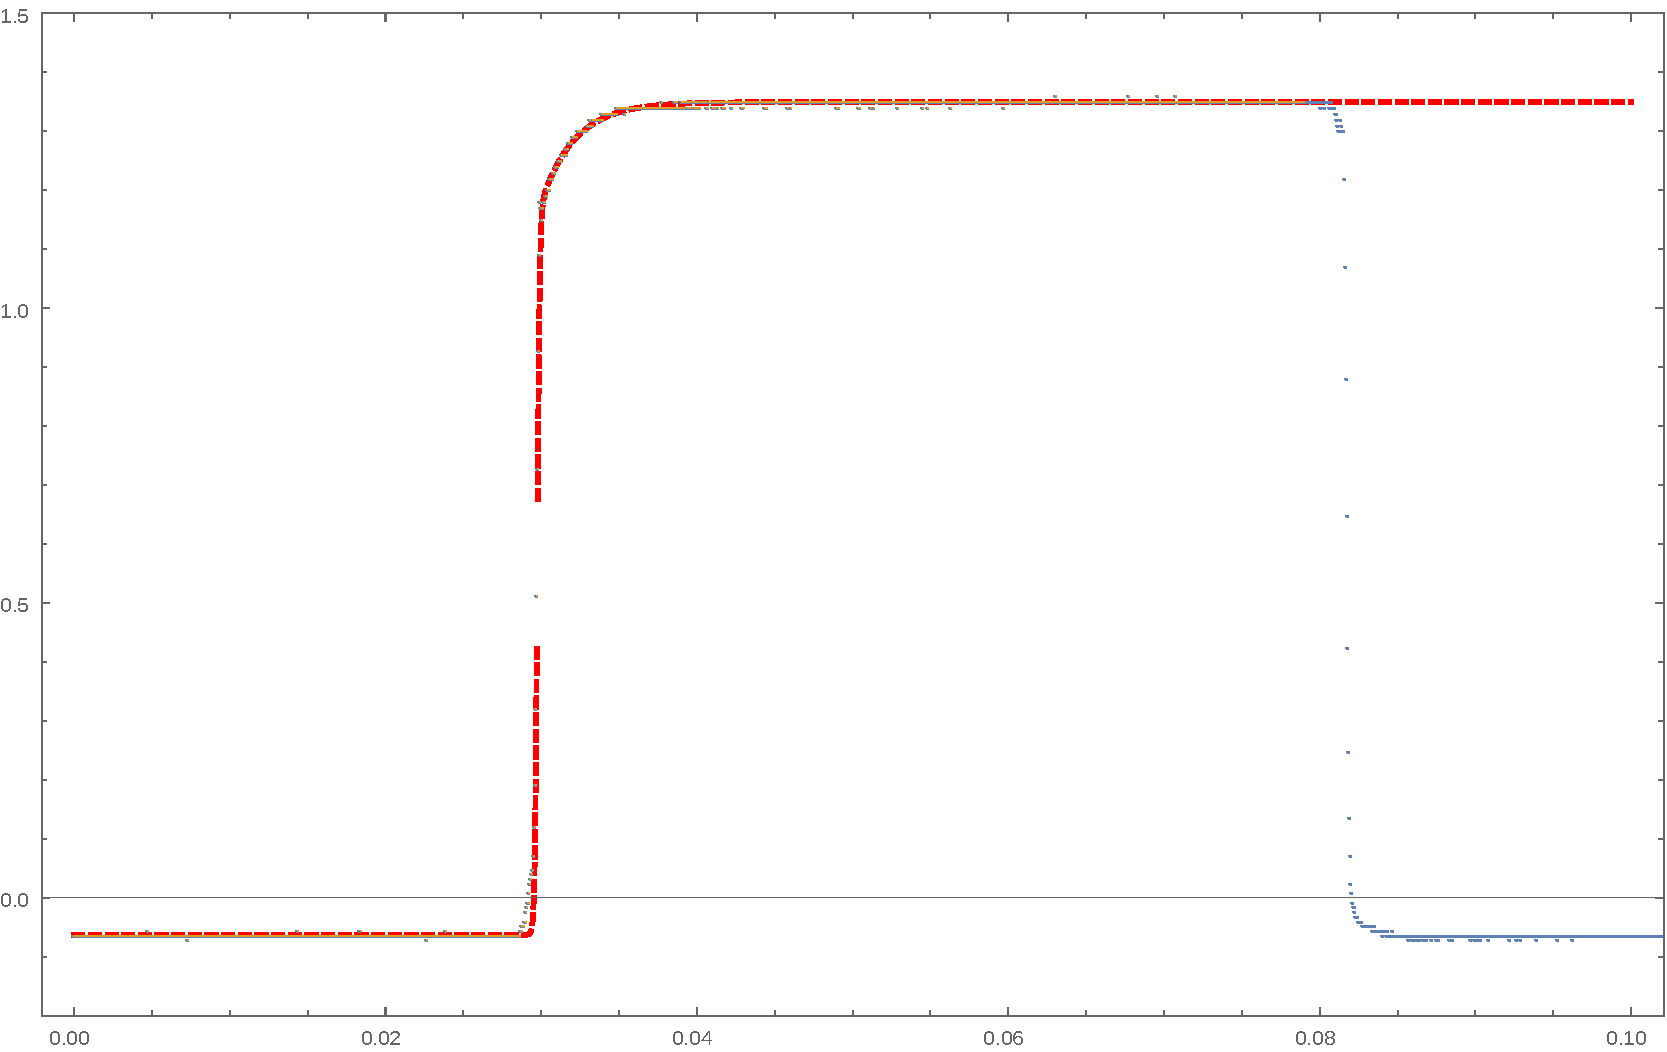
\includegraphics[width=0.7\textwidth]{../img/part6/exampletrans.pdf}
  \caption{Transmission der Rubidiumzelle bei Einschalten des Laserlichts und Fit mit $U(t)$.
  Die Höhe der Delle $B$ am Anfang des Plateaus ist abhängig von der vorangehenden Dunkelzeit $t_\text{d}$
  und enthält die Information über das Ausmaß der Relaxation im Dunklen.}
  \label{img:fra:exampletrans}
\end{center}
\end{figure}

Für die weitere Auswertung ist es notwendig, die Dunkelzeit $t_\text{d}$ zu bestimmen.
Die Methode dafür ist folgende:
Da die Chopperscheibe das Laserlicht mit einer Pulsweite von 50\% moduliert,
ist die Dunkelzeit genauso groß wie die Beleuchtungszeit.
Als Anfang der Beleuchtungszeit wird der gefittete Parameter $\mu$ verwendet.
Das Ende der Beleuchtungszeit $\mu'$ wird per Hand aus den Messdaten abgelesen
(es wird der Wert bei halber Transmission verwendet);
für den Fehler $s_{\mu'}$ auf die abgelesenen Werte wird 2\,ms angenommen.
Es gilt dann für die Dunkelzeit
\begin{equation}
  t_\text{d}=\mu'-\mu \ \, .
\end{equation}
%TODO richtiger Fehler auf Hellzeit

Eine Betrachtung der Fitergebnisse für die Verschmierung $\sigma$ der Fermi-Funktion
(\autoref{img:fra:sigmas}) zeigt,
warum es geeigneter ist, eine Fermi-Verteilung als Fitfunktion zu verwenden als ein
Rechtecksignal mit senkrechter Flanke:
Der nichtsenkrechte Anstieg des Rechtecksignals wird durch den Durchmesser des Laserstrahls verursacht, denn
der Strahl wird von der Chopperscheibe in einer kurzen Anstiegszeit geöffnet und nicht auf einmal.
Da die Anstiegszeit umgekehrt proportional zur Rotationsgeschwindigkeit der Scheibe und diese
wiederum umgekehrt proportional zur Dunkelzeit ist, erhält man einen linearen Zusammenhang
zwischen $\sigma$ und $t_\text{d}$.

Beim Experiment wurde versucht, die Anstiegszeit zu minimieren, indem der Chopper möglichst
nahe an die Laserdiode geschoben wurde, wo der Strahldurchmesser noch gering ist.

%TODO Bild sigmas root
\begin{figure}[H]
\begin{center}
  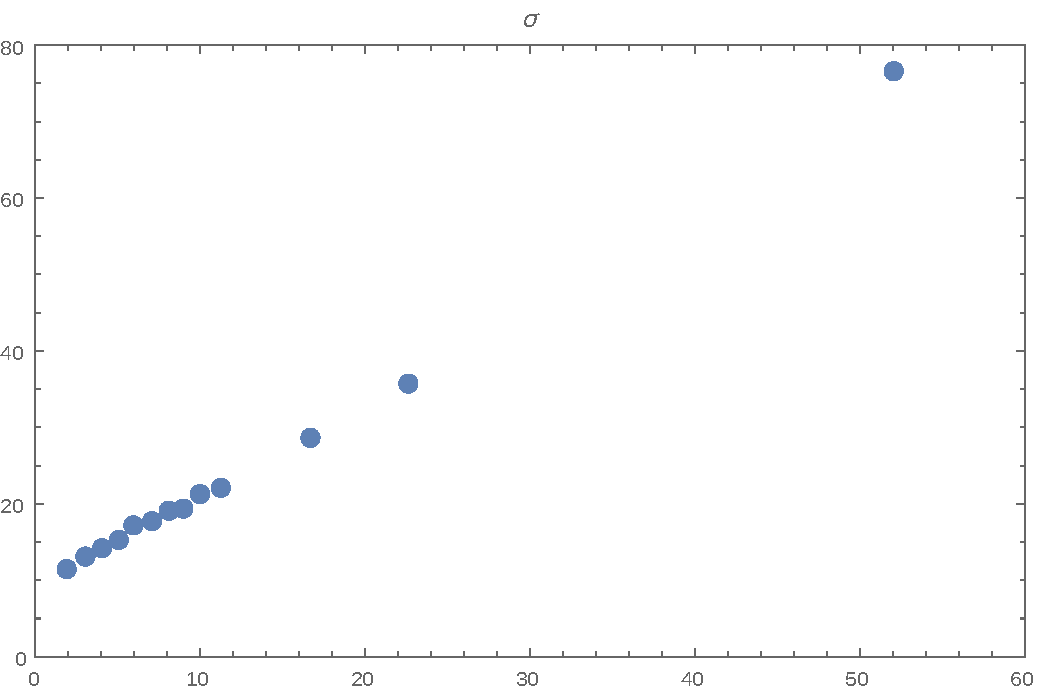
\includegraphics[width=0.6\textwidth]{../img/part6/sigmas.pdf}
  \caption{Verschmierung $\sigma$ der gefitteten Fermi-Funktionen in Abhängigkeit der Dunkelzeit $t_\text{d}$.
  Ursache für den linearen Zusammenhang ist die kleinere Rotationsgeschwindigkeit des Choppers bei
  größeren Dunkelzeiten.}
  \label{img:fra:sigmas}
\end{center}
\end{figure}

Der Wert für die Relaxationszeit $T_{\text{R}_\text{F}}$ kann aus den Fitdaten für den Parameter $B$ gewonnen werden.
Je größer die Dunkelzeit, desto länger kann das Ensemble relaxieren und $B$ ist dementsprechend größer.
Mit den Messungen bei unterschiedlichen Dunkelzeiten erhält
man daher Informationen über das Ausmaß der Relaxation zu
verschiedenen Zeitpunkten.
Die Relaxation folgt einem exponentiellen Gesetz; die Werte für $B$ werden daher mit
\begin{equation}
  B(t_\text{d})= a + b \cdot \left(1 - e^{-\frac{t_\text{d}}{T_{\text{R}_\text{F}}}}\right)
\end{equation}
gefittet.
\autoref{img:fra:Bs} zeigt diesen Fit. Der Parameter $a$ ist hier ein konstanter Offset,
$b$ beschreibt die Stärke der Relaxation bei großer Dunkelzeit und
$T_{\text{R}_\text{F}}$ die gesuchte Relaxationszeit nach Franzen.

%TODO Bild Bs root
\begin{figure}[H]
\begin{center}
  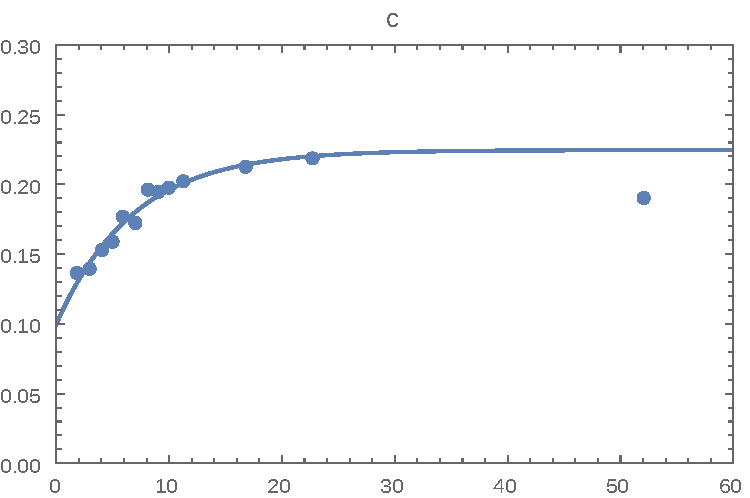
\includegraphics[width=0.6\textwidth]{../img/part6/Bs.pdf}
  \caption{Abhängigkeit des Fitparameters $B$ aus \autoref{eq:fra:fitfunct} von der Dunkelzeit $t_\text{d}$ und Fit
  mit einer exponentiellem Gesetz zur Bestimmung der Relaxationszeit $T_{\text{R}_\text{F}}$.}
  \label{img:fra:Bs}
\end{center}
\end{figure}

Der Fit liefert für die Relaxationszeit einen Wert von
\begin{equation}
  T_{\text{R}_\text{F}} = 6.8 \pm 1.2 \,\text{ms}
\end{equation}
und..
%TOTO richtige Fitergebnis für Trf, vgl mit litval.

